\section{Problem Analysis}

This section will expose several problems we took in account during the
initial phase of the project:

\begin{itemize}
\item \textbf{Domain Analysis}: description of the applicative context we
  considered to model
\item \textbf{Distribution}: since a need to distribute the system arises from
  the domain analysis, in this section we will discuss issues we encountered
  while designing the distribution of the city traffic simulator
\item \textbf{Concurrency}: it is reasonable to believe that some entities
  will act concurrently in the system, since the city traffic intrinsically
  contains more than one control unit\footnote{for control unit we mean each
  one of the single agents which represents a source of action}
\item \textbf{Application}: after outlining the domain of our simulations, we
  have to single out the major problems our level of abstraction entails
\item \textbf{Time}: finally we outline the questions we posed ourselves about
  the time flow during simulations
\end{itemize}

%%%%%%%%%%%%%%%%%%%%%%%%%%%%%%%%
%% DOMAIN ANALYSIS
%%%%%%%%%%%%%%%%%%%%%%%%%%%%%%%%

\subsection{Domain Analysis}\label{sec:pa-domain}
The goal of this project is to represent the traffic of a city. Among all the
different options we could choose, we decided to simulate some lively cities of
the United States of America (e.g., San Francisco).

Therefore, we can make some assumptions about this reality:

\begin{itemize}
\item the city is likely to have many commuters;
\item the city is likely to have many crossroads and traffic lights to
  regulate the traffic;
\item the city traffic can grow in certain days due to special events or
  recurrences;
\item cars are used mostly by a single person;
\item people mostly commute between two city spots, where we assume there
  will be a facility (a house, an office or something else) for each one;
\item the urban planning is Roman-like, i.e. streets have orthogonal
  intersections (\href{https://www.google.it/maps/place/San+Francisco,+California,+Stati+Uniti/@37.7766566,-122.4330836,16z/data=!4m2!3m1!1s0x80859a6d00690021:0x4a501367f076adff}{example}).
\end{itemize}

Even if our reference city\footnote{with the term \emph{``reference city"}
we are talking about a city which has similar characteristics to San
Francisco} has many means of transport, we will consider only a few meaningful
ones (besides \textbf{pedestrian} traffic): \textbf{bikes}, \textbf{cars} and
\textbf{buses}.

Every street segment could have sidewalks, bicycle paths and motor vehicles
lanes. In our reference city, road users must respect the following traffic
code:

\begin{itemize}
\item motor vehicles must stop in order to let pedestrians and bikes walk over
  respective zebra crossings;
\item each road user has to proceed in his/her street region: for example,
  pedestrians can not tread a road in the middle of a car lane unless it has a
  zebra crossing on it;
\item each crossroad will be regulated by traffic lights;
\item road users must not proceed faster than an eventual speed limit posted
  on a street segment;
\item vehicles can not enter a one-way in the wrong direction;
\item vehicles must give the way to other ones if it is requested by
  regulatory sign (STOP or YIELD);
\item vehicles must not turn in directions that are eventually forbidden by
  road signs;
\item vehicles must turn in directions that are eventually specified by road
  signs;
\item pedestrians and bikes cross street intersections ignoring traffic lights,
  since they just turn in the leftmost (rightmost) direction when they are on
  the left (right) side of the street.
\end{itemize}

Let us define exactly how we abstracted the structure of a city:

\begin{itemize}
  \item \textbf{Intersections} are either crossroads between three or four
    different roads
  \item We will call \textbf{street segment} the piece of road which lies
    between two consecutive intersections (i.e., a street segment touches
    \textit{exactly} two intersections). Since we will use frequently this
    component during the development of the simulator, we will simply refer to
    it as a \textit{street} for conciseness from now on.
    \begin{itemize}
      \item A street is composed of several ways. \textbf{Ways} are sets of
        adjacent lanes of the same type. A way can be a footway (i.e., a
        sidewalk), a bikeway or a roadway.
      \item A way is composed of lanes. \textbf{Lanes} are arrays of stretches
        treadable in just \textit{one} direction. A lane can be a footway lane,
        a bikeway lane or a roadway lane.
      \item A lane is made up of several stretches. A \textbf{stretch} is the
        basic structural unit of our reference city abstraction and, depending
        on the traveller type that can move on it (besides a few exceptions
        like zebra crossings), a stretch can be a footway stretch, a bikeway
        stretch or a roadway stretch.
    \end{itemize}
\end{itemize}

%%%%%%%%%%%%%%%%%%%%%%%%%%%%%%%%
%% DISTRIBUTION
%%%%%%%%%%%%%%%%%%%%%%%%%%%%%%%%

\subsection{Distribution}\label{sec:pa-distribution}
As we pointed out in section \ref{sec:pa-domain}, our system will be composed
of streets that are joined together by intersections.
Starting from this, we would like to distribute our system across several
computing nodes to attenuate the burden of running each simulation on single
nodes. We can do this by leveraging the knowledge we have at configuration time
about the geographical disposition of the structural macro-units of a city,
that is, street and intersections. In fact, we expect high interaction between
\textit{adjacent} structural macro-units.
More precisely, we will call \textbf{district} a set of streets and
intersections. Therefore, we will divide a city in districts and then we will
make them run in separated computing nodes.
% TODO: @Stefano, what do you say about the term "computing node"? Is it ok
%                 for a container?

Hence, in this section we will discuss about how we thought about distribution
issues.

\paragraph{Requirements} \mbox{} \\

In the following list we will express qualities our system should have to
effectively leverage distribution.

\begin{itemize}
\item The system should be distributed: we expect the simulator to manage many
  streets and much traffic. Thus, the system is probably going to handle load
  balancing in a better way if it allots partition of the city to different
  nodes rather than handing out all the load to a single node. This is
  specifically true in the case of special events, when the traffic load will
  greatly increase and the system must prove to be scalable
\item The system should appear as a single unit to its end user, in order to
  have an acceptable degree of transparency
\item The system might be composed of heterogeneous parts: whilst this issue
  is not mandatory, it makes the system more realistic
\item The system should be scalable: considering the nature of our project (a
  city simulator), we would like it to be scalable in possible directions
  (e.g., number of road users, city size, etc.)
\item The possibly scalable components of the system should be decoupled as
  much as possible from others
\item There should be a clearly defined protocol for the communication between
  each part of the system
\item When possible, the communication between two nodes of our system will be
  asynchronous: this quality leverages scalability
\item The system should boot/terminate consistently and ordered: with a fixed
  algorithm it is easier to ensure that all nodes are ready to execute/stop the
  system
\item The system should be able to save a consistent global state
\item The system should be fault tolerant, \emph{reactive} to possible faults
\item The system should be able to replicate and/or restore parts of itself,
  in order to be more fault tolerant
\item The system should be splitted in isolated parts, in order to isolate
  possible faults
\item The system should be able to locate each part of itself through a system
  of unique names
\item The replication/restoration operations should be transparent to the end
  user
\end{itemize}

\paragraph{Problems} \mbox{} \\

Several problems arose from this issues:

\begin{itemize}
\item How will we distribute our system?
\item How can we effectively boot the system in a neat and systematic manner?
\item How can we take a snapshot that is actually consistent in a distributed
  system?
\item How can we effectively shutdown the system in a neat and systematic
  manner?
\item The system might be seen in a control panel as if it were a film:
  \begin{itemize}
  \item what will it be able to show?
  \item will it offer different modalities an user can consume?
  \item how can we make the control panel see the traffic simulator as a
    single unit?
  \item will the stream show live events, deferred events or both?
  \end{itemize}
\item How can we set up an efficient and reliable naming resolution module?
\item How should we scatter the system across a set of nodes? How and which
  entities should we place in each node?
\item How errors will be managed by our system so that it can reach a certain
  degree of fault tolerancy?
\item How can we cope with well-known distributed systems network-related
  problems\footnote{considering \href{https://blogs.oracle.com/jag/resource/Fallacies.html?cm_mc_uid=82650292107114582847614&cm_mc_sid_50200000=1458564821}{The eight fallacies of distributed computing}: excluding the point 4,5,6
  since the topology of a city is statically defined and security issues are
  out of the project's scope}?
\item Are the answers at the previous questions providing a scalable solution?
\end{itemize}

%%%%%%%%%%%%%%%%%%%%%%%%%%%%%%%%
%% CONCURRENCY
%%%%%%%%%%%%%%%%%%%%%%%%%%%%%%%%

\subsection{Concurrency}\label{sec:pa-concurrency}
Looking at the applicative domain, there are several situations that inherently
express concurrent interactions between entities, for example more road users
that proceed in the same street segment.

We will show which concurrency issues we took into account during the beginning
of the project.

\paragraph{Requirements} \mbox{} \\

In the following list we will express qualities our system should have to
leverage concurrency.

\begin{itemize}
\item The system will present concurrency between some of its entities
\item The critical sections of each entity need to be identified
\item The critical sections of each entity  must be accessed in mutual
  exclusion
\item Time spent in critical sections will be reduced as much as possible
\item Blocking operations that are placed inside critical sections will be
  considered errors
\item We have to be able to show evidence of the fact that our system avoids
  deadlocks and livelocks
\item Causal dependencies between entities have to be outlined
\item Each valid state of an entity should be studied carefully so that
  protocols between entities operate in a correct way
\item Non-valid entity states should be pointed out so that we are able to
  think possible countermeasures to recover a preceeding valid state
\item Since in Section \ref{sec:pa-distribution} we express our willingness to
  be capable of obtaining consistent snapshots, each entity should provide a
  means to make a (possibly concurrent) dump of its internal state
\end{itemize}

\paragraph{Problems} \mbox{} \\

Concurrency requirements led us to make some questions about concurrency.

\begin{itemize}
\item How can we recognize that a situation is suitable to present concurrency?
\item How concurrent accesses will be managed? Will it make sense to discern
  side-effect accesses (\emph{procedures}) from read-only accesses
  (\emph{functions})?
\item Which entities have to be active? Which reactive? Which passive?
  \begin{itemize}
    \item Active entities perform actions according to their own will;
    \item Reactive entities are stateful and change their state in reaction to
      interaction with active entities;
    \item Passive entities are stateless.
  \end{itemize}
\item Should we use any formal technique to proof the correctness
of the system properties relating to concurrence?
\item Do we have the possibility to incur a non-valid state? If so, how do we
  handle the problem?
\item How can we avoid possible starvation scenarios?
\end{itemize}

%%%%%%%%%%%%%%%%%%%%%%%%%%%%%%%%
%% APPLICATION
%%%%%%%%%%%%%%%%%%%%%%%%%%%%%%%%

\subsection{Application Problems}\label{sec:pa-app-problems}

The way we abstracted city traffic bring new issues out and the way we can
resolve them is not straightforward.
We will use figure \ref{fig:pa-sample-street} and figure
\ref{fig:pa-sample-crossroad} to show examples in which tangled situations we
found out lie.

\begin{figure}[H]
  \centering
  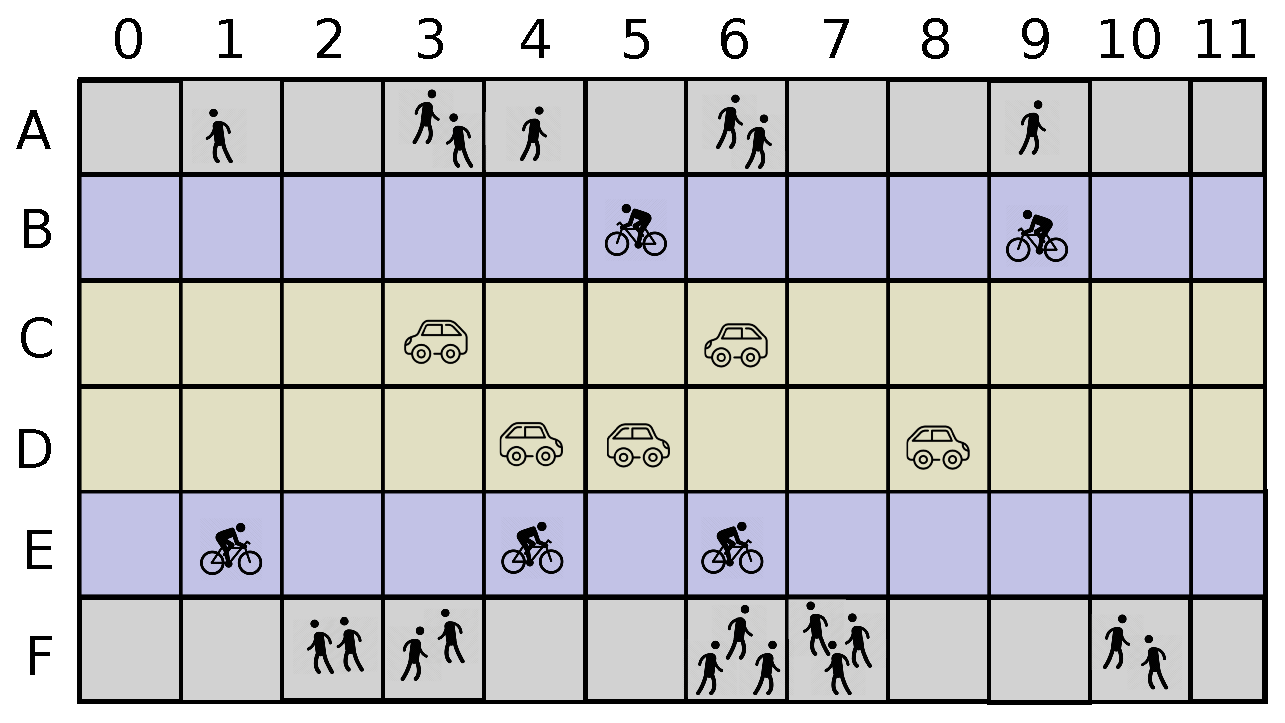
\includegraphics[width=.7\columnwidth]{images/analysis/street_base.eps}
  \caption{Sample street}
  \label{fig:pa-sample-street}
\end{figure}

\paragraph{Pedestrian Deadlock} \mbox{} \\

Let three be the maximum number of pedestrians in a sidewalk segment for the
sake of this example.
If we look at segments F6 and F7, there is a possible deadlock since
pedestrians in F6 can not proceed in an already full segment F7 and viceversa.

\paragraph{Rear-end Collisions} \mbox{} \\

Look at motor vehicles' lane segments D4 and D5. If car in D4 is going too
fast, there is a risk that it is going to collide with car in D5.

Thus, we will have to find a solution to avoid rear-end collisions.

\paragraph{Segment Parallelism} \mbox{} \\

It is realistic that some segments will be capable of containing more than one
road user, for example sidewalk segments.

As shown in figure \ref{fig:pa-sample-street}, there could be more road users
proceeding in the same direction (F2) or even in opposite directions (A3).

\begin{figure}[H]
  \centering
  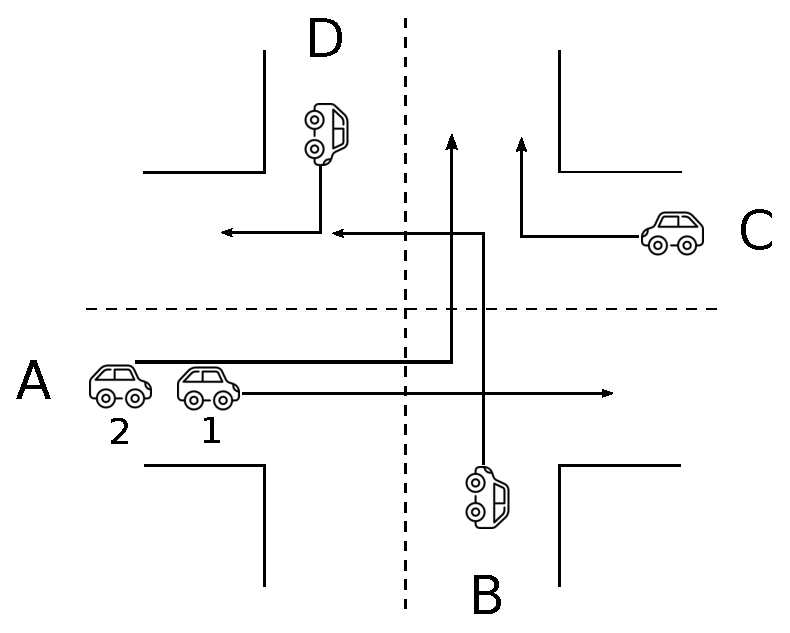
\includegraphics[width=.6\columnwidth]{images/analysis/crossroads.eps}
  \caption{Sample crossroad}
  \label{fig:pa-sample-crossroad}
\end{figure}

\paragraph{Zebra Crossings} \mbox{} \\

If there is a zebra crossing on a road segment, pedestrians (or bikes, if it
is a bike crossings) should be able to tread these stretches if they are free.
A concurrent attempt of another type of entity (e.g., car) to go over a
pedestrian crossing should be blocked so that the non-prioritized type of
entity would give the way to the privileged type of traveller (in our case,
the pedestrian).

\paragraph{Booking a Park Spot} \mbox{} \\

Even if it is an operation which might entail remote communication, the booking
of a park spot in another building will incur into concurrency issues when it
will be actually carried out.

In fact, there is a single garage out of which travellers are exiting, possibly
at the same time in which a remote booking operation is arriving. Therefore,
we will need to establish a protocol to regulate the dynamics of a garage.

\paragraph{Yield rules} \mbox{} \\

We will use \href{http://www.aci.it/i-servizi/normative/codice-della-strada/titolo-v-norme-di-comportamento/art-145-precedenza.html}{Italian yield rules}\footnote{we will also assume that vehicles proceed on the right side of the
street}, therefore if a vehicle's trajectory is met by another one from right,
the latter has to wait for the former to pass.
Looking at picture \ref{fig:pa-sample-crossroad}:
\begin{itemize}
    \item D is free to go since there is no vehicle on the right of its trajectory and so it is C;
    \item B must wait D to pass in order to turn left, whereas it does not have to wait
for C to turn right because B's and C's trajectories do not intersect;
    \item A.1 must wait for B to pass, while A.2 must wait for A.1, B and C.
\end{itemize}

%%%%%%%%%%%%%%%%%%%%%%%%%%%%%%%%
%% TIME
%%%%%%%%%%%%%%%%%%%%%%%%%%%%%%%%

\subsection{Time}\label{sec:pa-time-problems}
A traffic simulator is certainly appropriate for a real-time application.
Hence, we will strive to address in the most realistic way the following
issues:

\begin{itemize}
\item How can we simulate road users proceeding (regarding to travelling
  speed)?
\item How can we simulate crossroads (regarding to road users' arrivals time)?
\item How long do people stay in facilities for? How much precise do these
  intervals have to be?
\item How are semaphores going to be able to synchronize? Which of them decide
  how much time do they have to wait for?
\item When is it suitable to use logical clocks instead of local system clock?
\end{itemize}
